\input{../../plantillaexamen/preambuloexamen.tex}

\modulo{Redes de �rea Local.}
\tema {Examen del tema 5}



\pregunta{�Qu� es y para qu� se usa el TTL?.}{1}

\pregunta{Explica dos de las ventajas que supone dividir una red en subredes}{1}

\pregunta{Dada la m�scara 255.255.224.0 explica si podr� un equipo con la IP 45.28.84.101 comunicar con el 45.28.13.101.}{1}

\pregunta{Examina las tablas siguientes de tres router conectados en l�nea (A--B--C). Al router A llega un datagrama por la Interfaz FastEthernet 0/0 cuya direcci�n de destino es 161.63.45.81. Explica lo que ocurre a continuaci�n. Recuerda que 0.0.0.0 significa ``en cualquier otro caso''}{2}

\clearpage

\begin{table}[h]
	\centering
		\begin{tabular}{|c|c|c|}
			\hline
			Interfaz & FastEthernet 0/0 & IP: 1.0.0.1 \\
			\hline
			\hline
			Interfaz & FastEthernet 0/1 & IP: 2.0.0.1 \\
			\hline
			\hline
			10.0.0.0 & 255.255.255.0 & 1.0.0.2\\
			\hline 
			20.0.0.0 & 255.255.255.0 & 2.0.0.2\\
			\hline 
			161.63.45.0 & 255.255.255.0 & 2.0.0.2\\
			\hline 
			30.0.0.0 &  255.255.255.0 & 2.0.0.2\\
			\hline 
			40.0.0.0 &  255.255.255.0 & 1.0.0.2\\
			\hline
		\end{tabular}
	\caption{(Ejercicio 3) Configuracion del router A}
	\label{tab:Configuraciones}
\end{table}


\begin{table}[h]
	\centering
		\begin{tabular}{|c|c|c|}
			\hline
			Interfaz & FastEthernet 0/0 & IP: 2.0.0.2 \\
			\hline
			\hline
			Interfaz & FastEthernet 0/1 & IP: 3.0.0.1 \\
			\hline
			\hline
			10.0.0.0 & 255.255.255.0 & 2.0.0.1\\
			\hline 
			30.0.0.0 &  255.255.255.0 & 2.0.0.1\\
			\hline 
			40.0.0.0 &  255.255.255.0 & 1.0.0.2\\
			\hline
			0.0.0.0 & 255.255.255.255 & 3.0.0.2 \\
			\hline
		\end{tabular}
	\caption{(Ejercicio 3) Configuracion del router B}
	\label{tab:ConfiguracionesB}
\end{table}

\begin{table}[h]
	\centering
		\begin{tabular}{|c|c|c|}
			\hline
			Interfaz & FastEthernet 0/0 & IP: 3.0.0.2 \\
			\hline
			\hline
			Interfaz & FastEthernet 0/1 & IP: 4.0.0.1 \\
			\hline
			\hline
			10.0.0.0 & 255.255.255.0 & 3.0.0.1\\
			\hline 
			30.0.0.0 &  255.255.255.0 & 3.0.0.1\\
			\hline 
			40.0.0.0 &  255.255.255.0 & 3.0.0.1\\
			\hline
			0.0.0.0 & 255.255.255.255 & 3.0.0.1 \\
			\hline
		\end{tabular}
	\caption{(Ejercicio 3) Configuracion del router C}
	\label{tab:ConfiguracionesB}
\end{table}

\pregunta{Una empresa tiene cuatro sedes con cuatro routers A, B, C y D conectados en forma de cuadrado y con enrutamiento est�tico. En cada sede los prefijos asignados son:
\begin{itemize}
	\item 10.0.0.0/24 para la sede A
	\item 20.0.0.0/24 para la sede B
	\item 30.0.0.0/24 para la sede C
	\item 40.0.0.0/24 para la sede D
\end{itemize}
Aparte de eso las conexiones entre router son como se indican:
\begin{itemize}
	\item Tarjeta 0/0 de A con la tarjeta 0/0 de B (subred 1.0.0.0).
	\item Tarjeta 0/1 de A con la tarjeta 0/1 de C.(subred 2.0.0.0)
	\item Tarjeta 0/0 de C con la tarjeta 0/0 de D. (subred 3.0.0.0)
	\item Tarjeta 0/1 de D con la tarjeta 0/1 de B. (subred 4.0.0.0)
	\item Tarjeta 0/1/0 de A con el switch de la sede A.
	\item Tarjeta 0/1/0 de B con el switch de la sede B.
	\item Tarjeta 0/1/0 de C con el switch de la sede C.
	\item Tarjeta 0/1/0 de D con el switch de la sede D.
\end{itemize}
Rellena las tablas adjuntas con las IP, las rutas y los comandos Cisco correspondientes. Sup�n que el prompt que se ve es {\ttfamily Router(config)\#} y que no hace falta que escribas {\ttfamily exit}.
}{3}



\pregunta{Una red de routers est� interconectada como muestra el dibujo. Los costes asociados a los distintos enlaces son los que se muestran en las l�neas. Todos ellos han sido configurados con OSPF para poder disponer de autoconfiguraci�n de rutas. Se desea saber como progresa el algoritmo OSPF para encontrar el mejor camino desde el router A al router I.
}{2}
\begin{figure}[b]
	\centering
		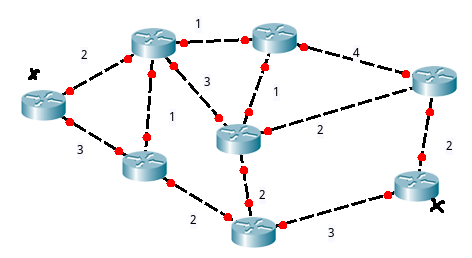
\includegraphics[width=0.95\textwidth]{ospf.png}
	\label{fig:ospf}
\end{figure}

\fin
\end{document}

